\documentclass[11pt]{article}
\usepackage{listings}
\usepackage{pgf}
\usepackage{tikz}
\usepackage{alltt}
\usepackage{hyperref}
\usepackage{url}
\usepackage{amssymb}
\usetikzlibrary{arrows,automata,shapes,positioning}
\tikzstyle{block} = [rectangle, draw, fill=blue!20, 
    text width=5em, text centered, rounded corners, minimum height=2em]
\tikzstyle{bt} = [rectangle, draw, fill=blue!20, 
    text width=1em, text centered, rounded corners, minimum height=2em]

\newtheorem{defn}{Definition}
\newtheorem{crit}{Criterion}
\newcommand{\true}{\mbox{\sf true}}
\newcommand{\false}{\mbox{\sf false}}

\newcommand*\circled[1]{\tikz[baseline=(char.base)]{
            \node[shape=circle,draw,inner sep=2pt] (char) {#1};}}


\newcommand{\handout}[5]{
  \noindent
  \begin{center}
  \framebox{
    \vbox{
      \hbox to 5.78in { {\bf Software Testing, Quality Assurance and Maintenance } \hfill #2 }
      \vspace{4mm}
      \hbox to 5.78in { {\Large \hfill #5  \hfill} }
      \vspace{2mm}
      \hbox to 5.78in { {\em #3 \hfill #4} }
    }
  }
  \end{center}
  \vspace*{4mm}
}

\newcommand{\lecture}[4]{\handout{#1}{#2}{#3}{#4}{Lecture #1}}
\topmargin 0pt
\advance \topmargin by -\headheight
\advance \topmargin by -\headsep
\textheight 8.9in
\oddsidemargin 0pt
\evensidemargin \oddsidemargin
\marginparwidth 0.5in
\textwidth 6.5in

\parindent 0in
\parskip 1.5ex
%\renewcommand{\baselinestretch}{1.25}

\usepackage{enumitem}

\newtheorem{prop}{Proposition}
\newtheorem{lemma}{Lemma}
\usepackage{ebproof}
\newcommand{\qedsymbol}{\rule{1ex}{1ex}}

\lstset{ %
language=Java,
basicstyle=\ttfamily,commentstyle=\scriptsize\itshape,showstringspaces=false,breaklines=true,numbers=left}

%\usepackage{fontspec}
%\setmonofont{Cousine}[Scale=MatchLowercase]

\begin{document}

\lecture{9 --- February 3, 2025}{Winter 2025}{Patrick Lam}{version 1}

We've talked about symbolic execution, which seems too good to be true, from the examples that we saw.
What? Automatically finding inputs that explore all interesting behaviour? How?

The issue with symbolic executiion is that it's hard to scale. Consider these three problems.
\begin{enumerate}[noitemsep]
\item Code that's hard to analyze: for instance, think of a cryptographic hash function. Smart people have tried to understand how they do what they do. Symbolic execution won't be able to analyze it.
\item Path explosion: the number of paths grows exponentially with the number of nested if statements; handling function calls can also lead to exponential growth; and loops can simply be unbounded.
\item Environment: in the examples we saw, the input was just integers. But in general there might be data structures (and pointers); files and databases; the network, and sockets; and threads (you need to explore all thread schedules).
\end{enumerate}

\paragraph{Example.} Here's a bit of a contrived example.
\begin{lstlisting}
  int obscure(int x, int y) {
    if (x == complex(y))
      error();
    return 0;
  }
\end{lstlisting}
Recall that symbolic execution is trying to find inputs that reach all
program points, including the call to \texttt{error()}.  So, it
considers the \texttt{if} condition \texttt{x == complex(y)}. In the
previous lecture, we had conditions that were just simple arithmetic
and boolean expressions, and hence easy to make either true or false
(by changing the values of the variables in the expressions), using an
SMT solver.  Now, it has to find values for \texttt{x} and \texttt{y}
such that (in this case) \texttt{x == complex(y)}. But
\texttt{complex()} is opaque to the SMT solver, and can be arbitrarily
complicated.

\begin{itemize}[noitemsep]
\item Who is being called? We see \texttt{complex()} here, but that could be
  a virtual function (\texttt{this.complex()}) and we don't necessarily know the
  runtime type of \texttt{this}. Or, it could be a function pointer.
\item Function \texttt{complex()} could be a cryptographic function, like a password hash.
  Now you have to find a password that matches a given hash. Good luck!
\item \texttt{complex()} could contain non-linear integer or floating point arithmetic,
  hard for SMT solvers to reason about.
\item \texttt{complex()} could contain system calls, file I/O, network I/O, etc.
\end{itemize}

\section*{Dynamic Symbolic Execution (DSE)}
We have some tools to mitigate the obstacles to symbolic execution,
under the general name of ``dynamic symbolic execution''.  Symbolic
execution operates completely on symbolic inputs ($X$, $Y$), not
concrete inputs (numbers $17$, $5$).  But sometimes that's hard or
impossible. We thus aim to use concrete execution (as formalized in
the operational semantics) when symbolic execution is hard. The
concrete execution will hopefully guide symbolic execution to useful
parts of the code. This approach is therefore also known as a
\emph{concolic testing} (``\textbf{conc}rete'' +
``symb\textbf{olic}'').

Let's see how it works. Here's the program again.

\begin{lstlisting}
  int obscure(int x, int y) {
    if (x == complex(y))
      error();
    return 0;
  }
\end{lstlisting}
One of the approaches to dynamic symbolic execution is called DART,
for Directed Automated Random Testing. 

\paragraph{Run 1.} So, we'll start with some random inputs.
Let \texttt{x=33} and \texttt{y=42}, which are concrete values you
generated randomly. You concretely run \texttt{complex(42)} and find
that it returns concrete value 567. Since $33 \neq 567$, these inputs lead to the else
branch.

OK, now we want to explore the then-branch. Symbolic execution wants to negate the
\texttt{if}-condition. Oops, that's too hard. Let's instead try running again.
What \texttt{x} should we use? Why not \texttt{x=567}?

\paragraph{Run 2.} This time we are trying with \texttt{x=567} and \texttt{y=42},
as indicated by the previous run. It turns out that \texttt{complex(42)} still returns
567 (it didn't have to, but it does). So the execution goes to the then branch,
covering all branches, and finding the error.

\subsection*{Flavours of Symbolic Execution}
In the previous lecture, we talked about \emph{static symbolic execution} (or classical symbolic execution).
\begin{itemize}[noitemsep]
\item simulates execution on program source code (with symbolic values)
\item starts from entry point, computes strongest post-conditions (symbolically) for the method (by computing them for every program point).
\end{itemize}
Now, we're talking about \emph{dynamic symbolic execution}.
\begin{itemize}[noitemsep]
    \item run/interpret program with concrete state (concrete values)
    \item in parallel, also compute symbolic state alongside concrete state (``concolic'')
    \item occasionally, SMT solver generates new concrete inputs, increasing coverage.
\end{itemize}
Note that the notion of path coverage is key here. We're aiming to increase it.

There are two main flavours of DSE:
\begin{itemize}[noitemsep]
\item EXE-style~\cite{cadar06:_exe}: tools include KLEE (Imperial College London), SPF (NASA), Cloud9, S2E (EPFL)
  \item DART-style~\cite{godefroid05:_dart}: tools include SAGE, PEX (Microsoft), CUTE (UIUC), CREST (UC Berkeley)
\end{itemize}
More on the differences between these later.

\section{EXE}
Let's start by seeing how the EXE-style dynamic symbolic execution works.

\paragraph{Overview.} First, as with the example run we saw before, EXE runs the program concretely, with concrete inputs. You might use fuzzing
or just hard-code some initial inputs.

But, at the same time, EXE runs the symbolic execution in parallel. The symbolic execution follows the concrete execution,
keeping track of which values are inputs (symbolic) or not inputs (concrete). We've talked about computing path conditions
before, and we'll do that here, in terms of the symbolic inputs.

Things get interesting at branch points, where our goal is to explore both cases. At every branch point:
\begin{itemize}[noitemsep]
\item concrete execution will take a branch, say branch1.
\item symbolic execution then forces execution into branch2 as well; it updates the input to do that, updating the path condition, and hence creating a new concrete state that reaches branch2.
\end{itemize}
We now have concrete inputs that reach both branch1 and branch2.

\paragraph{Details.} For dynamic symbolic execution, a program state contains a path condition $\mathit{pc}$, as well as values for all variables.
Variables always have a concrete value (in our formalization, an integer), and may have a symbolic value as well (an expression which may contain
input variables e.g. $X$). To start, the state contains mappings to symbolic state like $\mathtt{x}=X$ for all inputs $X$.

At each execution step:
\begin{itemize}[noitemsep]
\item update the concrete state by executing a program instruction concretely;
\item update the symbolic state by executing the same instruction symbolically;
\item if the instruction is a branch:
  \begin{itemize}
    \item fork the execution state into two
    \item true branch: conjoin the branch condition to the previous path condition
    \item false branch: conjoin the negated branch condition to the previous path condition (that's how you get in the else branch)
    \item for the branch that the concrete execution didn't take, ask the SMT solver to compute new initial concrete values from the symbolic state. These new inputs must be consistent with the relevant path condition. Replace concrete values with the newly-computed ones, obtaining them by substituting the new inputs into the symbolic state. (Possibly this is impossible, in which case you give up on that path.)
  \end{itemize}
\end{itemize}
Let's look at an example. One could do this example with classical symbolic execution, but let's do EXE-style on it.
\begin{lstlisting}
  int proc(int x) {
    int r = 0;

    if (x > 8) { // (1)
      r = x - 7
    }

    if (x < 5) { // (2)
      r = x - 2;
    }
  }
\end{lstlisting}

Here's our initial state.


\begin{center}
    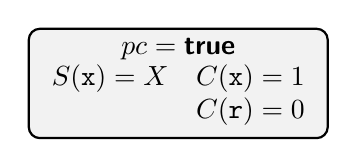
\begin{tikzpicture}[
        node distance=1.5cm and 1cm,
        every node/.style={draw, rounded corners, fill=gray!10, align=center},
        every path/.style={thick},
        decision/.style={draw, rounded corners, fill=gray!20, align=center, minimum width=3.5cm}
    ]


    % Nodes
      \node (start) {\textbf{$pc = \textsf{true}$} \\
        $\begin{array}{ll}
        S(\mathtt{x}) = X & C(\mathtt{x}) = 1 \\
                          & C(\mathtt{r}) = 0
      \end{array}$ };
    
    
    \end{tikzpicture}
\end{center}
The start of the method is always reachable, so \textbf{$pc = \textsf{true}$}. There is one input $X$,
so we have symbolic state $S(\mathtt{x}) = X$. We also have an arbitrarily-drawn concrete value for
\texttt{x}, which is 1, and \texttt{r} will be 0 soon enough.

Let's start executing the program. We have a branch at (1) on condition
$\texttt{x} > 8$. The concrete state $\texttt{x}=1$ drives the concrete execution
into the else branch, indicated by the dotted line.

\begin{center}
    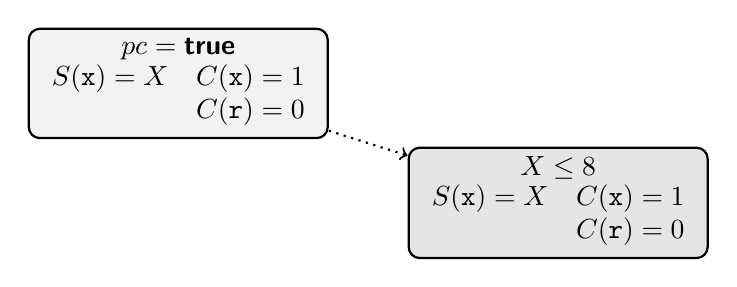
\begin{tikzpicture}[
        node distance=1.5cm and 1cm,
        every node/.style={draw, rounded corners, fill=gray!10, align=center},
        every path/.style={thick},
        decision/.style={draw, rounded corners, fill=gray!20, align=center, minimum width=3.5cm, yshift=2em}
    ]


    % Nodes
      \node (start) {\textbf{$pc = \textsf{true}$} \\
        $\begin{array}{ll}
        S(\mathtt{x}) = X & C(\mathtt{x}) = 1 \\
                          & C(\mathtt{r}) = 0
      \end{array}$ };
    
    \node (right)[below right=of start, decision,yshift=2em] {$X \leq 8$ \\ 
        $\begin{array}{ll}
        S(\mathtt{x}) = X & C(\mathtt{x}) = 1 \\
                          & C(\mathtt{r}) = 0
      \end{array}$ };
    \draw[->, dotted] (start) -- (right);
    
    \end{tikzpicture}
\end{center}
Now we also visit the then-branch. The path condition is simply the branch condition $X > 8$.
We ask the SMT solver to generate a value for $X$ that satisfies $X > 8$; it can ($\checkmark$), and comes back with 9 for $X$
and hence \texttt{x}.
We don't update \texttt{r} since it doesn't depend on $X$.

\begin{center}
    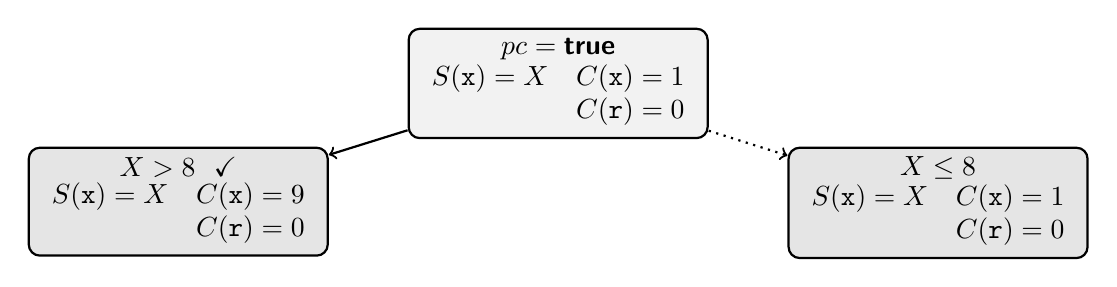
\begin{tikzpicture}[
        node distance=1.5cm and 1cm,
        every node/.style={draw, rounded corners, fill=gray!10, align=center},
        every path/.style={thick},
        decision/.style={draw, rounded corners, fill=gray!20, align=center, minimum width=3.5cm, yshift=2em}
    ]


    % Nodes
      \node (start) {\textbf{$pc = \textsf{true}$} \\
        $\begin{array}{ll}
        S(\mathtt{x}) = X & C(\mathtt{x}) = 1 \\
                          & C(\mathtt{r}) = 0
      \end{array}$ };
    
    \node (left)[below left=of start, decision,yshift=2em] {$X > 8 ~~ \checkmark$ \\ 
        $\begin{array}{ll}
        S(\mathtt{x}) = X & C(\mathtt{x}) = 9 \\
                          & C(\mathtt{r}) = 0
      \end{array}$ };
    \node (right)[below right=of start, decision,yshift=2em] {$X \leq 8$ \\ 
        $\begin{array}{ll}
        S(\mathtt{x}) = X & C(\mathtt{x}) = 1 \\
                          & C(\mathtt{r}) = 0
      \end{array}$ };
    
    % Edges
    \draw[->] (start) -- (left);
    \draw[->, dotted] (start) -- (right);
    
    \end{tikzpicture}
\end{center}
We continue execution on the then-branch, which reassigns \texttt{r}.
\begin{center}
    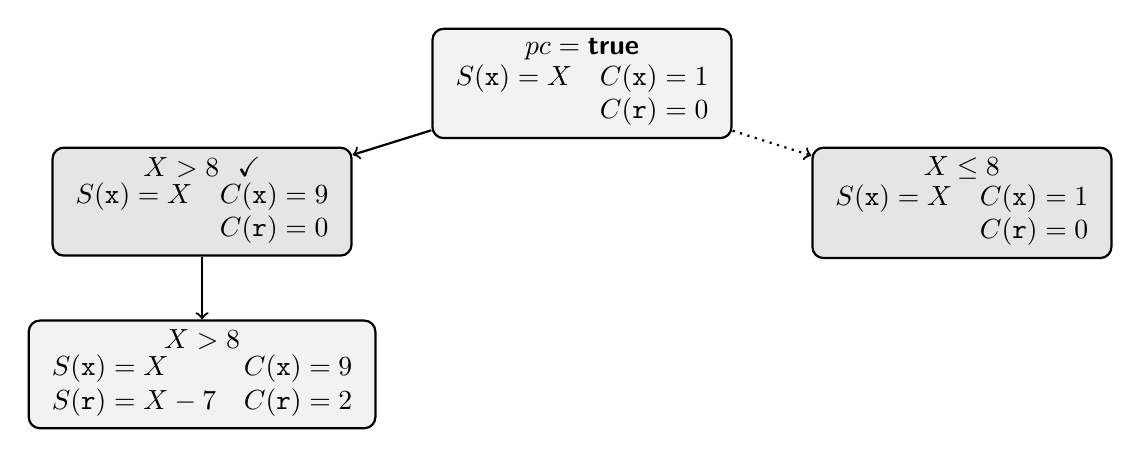
\begin{tikzpicture}[
        node distance=1.5cm and 1cm,
        every node/.style={draw, rounded corners, fill=gray!10, align=center},
        every path/.style={thick},
        decision/.style={draw, rounded corners, fill=gray!20, align=center, minimum width=3.5cm, yshift=2em}
    ]


    % Nodes
      \node (start) {\textbf{$pc = \textsf{true}$} \\
        $\begin{array}{ll}
        S(\mathtt{x}) = X & C(\mathtt{x}) = 1 \\
                          & C(\mathtt{r}) = 0
      \end{array}$ };
    
    \node (left)[below left=of start, decision,yshift=2em] {$X > 8 ~~ \checkmark$ \\ 
        $\begin{array}{ll}
        S(\mathtt{x}) = X & C(\mathtt{x}) = 9 \\
                          & C(\mathtt{r}) = 0
      \end{array}$ };
    \node (left2)[below=of left,yshift=2em] {$X > 8$ \\ 
        $\begin{array}{ll}
        S(\mathtt{x}) = X & C(\mathtt{x}) = 9 \\
        S(\mathtt{r}) = X - 7 & C(\mathtt{r}) = 2
      \end{array}$ };
    \node (right)[below right=of start, decision,yshift=2em] {$X \leq 8$ \\ 
        $\begin{array}{ll}
        S(\mathtt{x}) = X & C(\mathtt{x}) = 1 \\
                          & C(\mathtt{r}) = 0
      \end{array}$ };
    
    % Edges
    \draw[->] (start) -- (left);
    \draw[->] (left) -- (left2);
    \draw[->, dotted] (start) -- (right);
    
    \end{tikzpicture}
\end{center}
Let's continue with the next if-statement (2). In this case we have concrete \texttt{x} being 9, which runs to the else-branch, and finishes with no further changes in state.
\begin{center}
    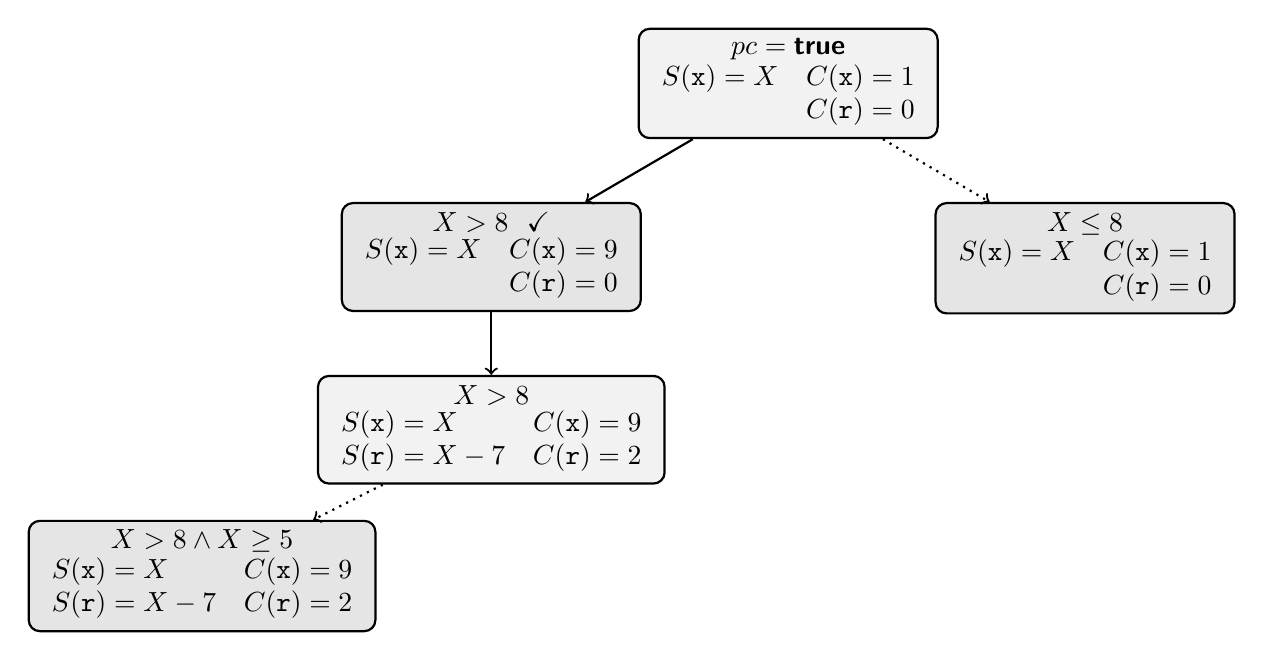
\begin{tikzpicture}[
        node distance=1.5cm and 1cm,
        every node/.style={draw, rounded corners, fill=gray!10, align=center},
        every path/.style={thick},
        decision/.style={draw, rounded corners, fill=gray!20, align=center, minimum width=3.5cm, yshift=2em}
    ]


    % Nodes
      \node (start) {\textbf{$pc = \textsf{true}$} \\
        $\begin{array}{ll}
        S(\mathtt{x}) = X & C(\mathtt{x}) = 1 \\
                          & C(\mathtt{r}) = 0
      \end{array}$ };
    
    \node (left)[below left=of start, decision,xshift=3em] {$X > 8 ~~ \checkmark$ \\ 
        $\begin{array}{ll}
        S(\mathtt{x}) = X & C(\mathtt{x}) = 9 \\
                          & C(\mathtt{r}) = 0
      \end{array}$ };
    \node (left2)[below=of left,yshift=2em] {$X > 8$ \\ 
        $\begin{array}{ll}
        S(\mathtt{x}) = X & C(\mathtt{x}) = 9 \\
        S(\mathtt{r}) = X - 7 & C(\mathtt{r}) = 2
      \end{array}$ };
    \node (left3)[below left=of left2,decision,xshift=5em,yshift=1em] {$X > 8 \wedge X \ge 5$ \\ 
        $\begin{array}{ll}
        S(\mathtt{x}) = X & C(\mathtt{x}) = 9 \\
        S(\mathtt{r}) = X - 7 & C(\mathtt{r}) = 2
      \end{array}$ };
    
    \node (right)[below right=of start, decision,xshift=-3em] {$X \leq 8$ \\ 
        $\begin{array}{ll}
        S(\mathtt{x}) = X & C(\mathtt{x}) = 1 \\
                          & C(\mathtt{r}) = 0
      \end{array}$ };
    
    % Edges
    \draw[->] (start) -- (left);
    \draw[->] (left) -- (left2);
    \draw[->,dotted] (left2) -- (left3);
    \draw[->, dotted] (start) -- (right);
    
    \end{tikzpicture}
\end{center}
The other possibility is the then-branch of (2). Let's try that.
\begin{center}
    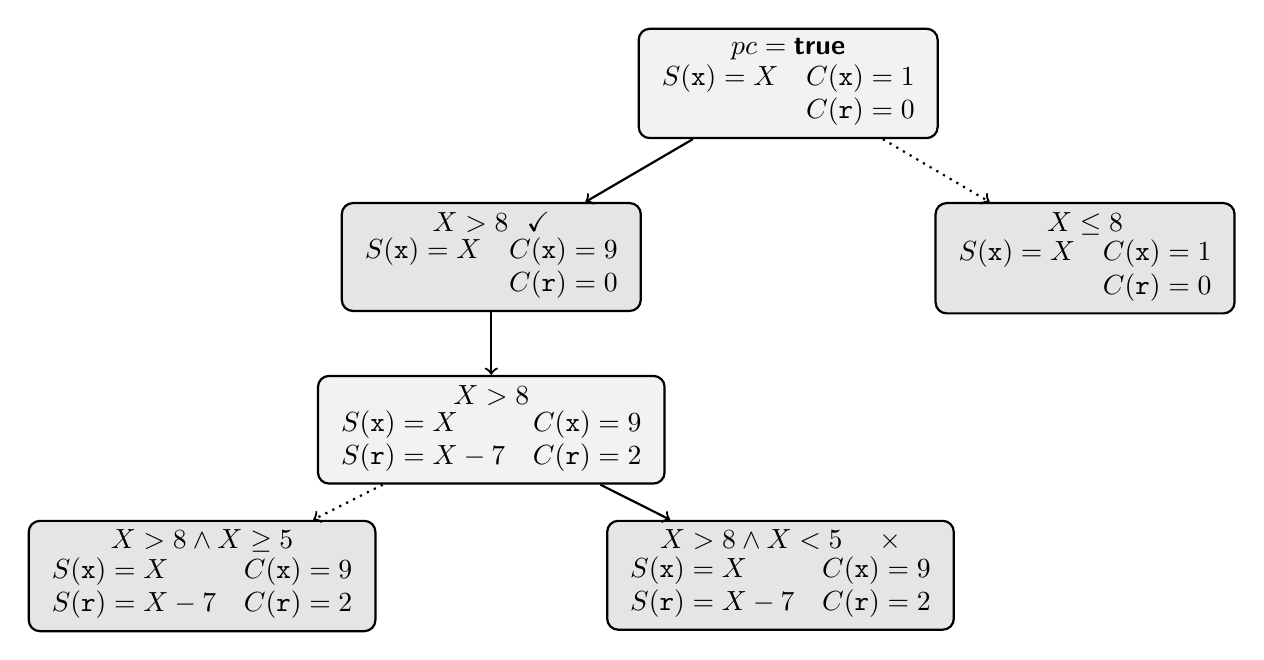
\begin{tikzpicture}[
        node distance=1.5cm and 1cm,
        every node/.style={draw, rounded corners, fill=gray!10, align=center},
        every path/.style={thick},
        decision/.style={draw, rounded corners, fill=gray!20, align=center, minimum width=3.5cm, yshift=2em}
    ]


    % Nodes
      \node (start) {\textbf{$pc = \textsf{true}$} \\
        $\begin{array}{ll}
        S(\mathtt{x}) = X & C(\mathtt{x}) = 1 \\
                          & C(\mathtt{r}) = 0
      \end{array}$ };
    
    \node (left)[below left=of start, decision,xshift=3em] {$X > 8 ~~ \checkmark$ \\ 
        $\begin{array}{ll}
        S(\mathtt{x}) = X & C(\mathtt{x}) = 9 \\
                          & C(\mathtt{r}) = 0
      \end{array}$ };
    \node (left2)[below=of left,yshift=2em] {$X > 8$ \\ 
        $\begin{array}{ll}
        S(\mathtt{x}) = X & C(\mathtt{x}) = 9 \\
        S(\mathtt{r}) = X - 7 & C(\mathtt{r}) = 2
      \end{array}$ };
    \node (left3)[below left=of left2,decision,xshift=5em,yshift=1em] {$X > 8 \wedge X \ge 5$ \\ 
        $\begin{array}{ll}
        S(\mathtt{x}) = X & C(\mathtt{x}) = 9 \\
        S(\mathtt{r}) = X - 7 & C(\mathtt{r}) = 2
      \end{array}$ };
    \node (left3b)[below right=of left2,decision,xshift=-5em,yshift=1em] {$X > 8 \wedge X < 5$ ~~ $\times$ \\ 
        $\begin{array}{ll}
        S(\mathtt{x}) = X & C(\mathtt{x}) = 9 \\
        S(\mathtt{r}) = X - 7 & C(\mathtt{r}) = 2
      \end{array}$ };
    
    \node (right)[below right=of start, decision,xshift=-3em] {$X \leq 8$ \\ 
        $\begin{array}{ll}
        S(\mathtt{x}) = X & C(\mathtt{x}) = 1 \\
                          & C(\mathtt{r}) = 0
      \end{array}$ };
    
    % Edges
    \draw[->] (start) -- (left);
    \draw[->] (left) -- (left2);
    \draw[->,dotted] (left2) -- (left3);
    \draw[->] (left2) -- (left3b);
    \draw[->, dotted] (start) -- (right);
    
    \end{tikzpicture}
\end{center}
We have an unsatisfiable path condition $X > 8 \wedge X < 5$ so we give up.

We've now completely explored the then-branch of (1). We still haven't finished
exploring the else-branch of (1), so we continue executing it until we reach (2).
In this case, the concrete state says to execute the then-branch of (2).
\begin{center}
    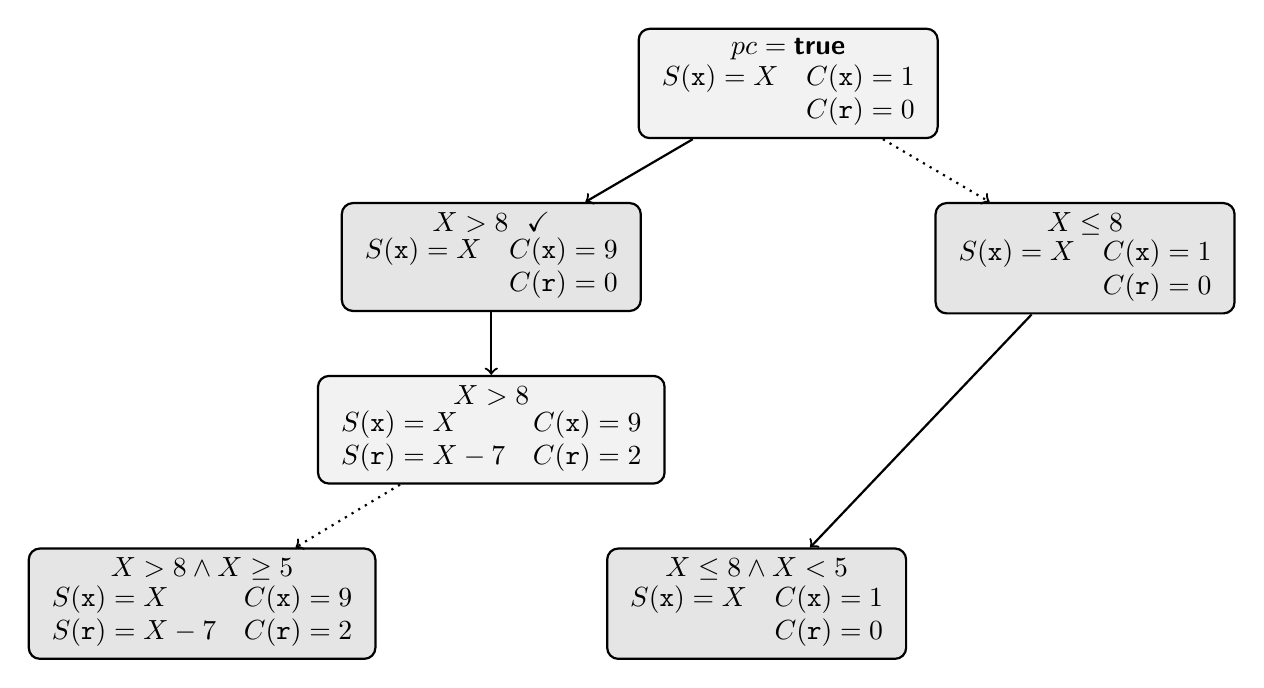
\begin{tikzpicture}[
        node distance=1.5cm and 1cm,
        every node/.style={draw, rounded corners, fill=gray!10, align=center},
        every path/.style={thick},
        decision/.style={draw, rounded corners, fill=gray!20, align=center, minimum width=3.5cm, yshift=2em}
    ]


    % Nodes
      \node (start) {\textbf{$pc = \textsf{true}$} \\
        $\begin{array}{ll}
        S(\mathtt{x}) = X & C(\mathtt{x}) = 1 \\
                          & C(\mathtt{r}) = 0
      \end{array}$ };
    
    \node (left)[below left=of start, decision,xshift=3em] {$X > 8 ~~ \checkmark$ \\ 
        $\begin{array}{ll}
        S(\mathtt{x}) = X & C(\mathtt{x}) = 9 \\
                          & C(\mathtt{r}) = 0
      \end{array}$ };
    \node (left2)[below=of left,yshift=2em] {$X > 8$ \\ 
        $\begin{array}{ll}
        S(\mathtt{x}) = X & C(\mathtt{x}) = 9 \\
        S(\mathtt{r}) = X - 7 & C(\mathtt{r}) = 2
      \end{array}$ };
    \node (left3)[below left=of left2,decision,xshift=5em] {$X > 8 \wedge X \ge 5$ \\ 
        $\begin{array}{ll}
        S(\mathtt{x}) = X & C(\mathtt{x}) = 9 \\
        S(\mathtt{r}) = X - 7 & C(\mathtt{r}) = 2
      \end{array}$ };
    
    \node (right)[below right=of start, decision,xshift=-3em] {$X \leq 8$ \\ 
        $\begin{array}{ll}
        S(\mathtt{x}) = X & C(\mathtt{x}) = 1 \\
                          & C(\mathtt{r}) = 0
      \end{array}$ };
    \node (right2)[below right=of left2,decision,xshift=-5em] {$X \le 8 \wedge X < 5$ \\ 
        $\begin{array}{ll}
        S(\mathtt{x}) = X & C(\mathtt{x}) = 1 \\
                          & C(\mathtt{r}) = 0
      \end{array}$ };
    
    % Edges
    \draw[->] (start) -- (left);
    \draw[->] (left) -- (left2);
    \draw[->,dotted] (left2) -- (left3);
    \draw[->] (right) -- (right2);
    \draw[->, dotted] (start) -- (right);
    
    \end{tikzpicture}
\end{center}
Let's put that on hold for now and explore the else-branch of (2). Here we falsify its branch condition
and successfully $(\checkmark)$ find $X = 6$ as a solution to that path constraint, thus setting $\texttt{x} = 6$.
\begin{center}
    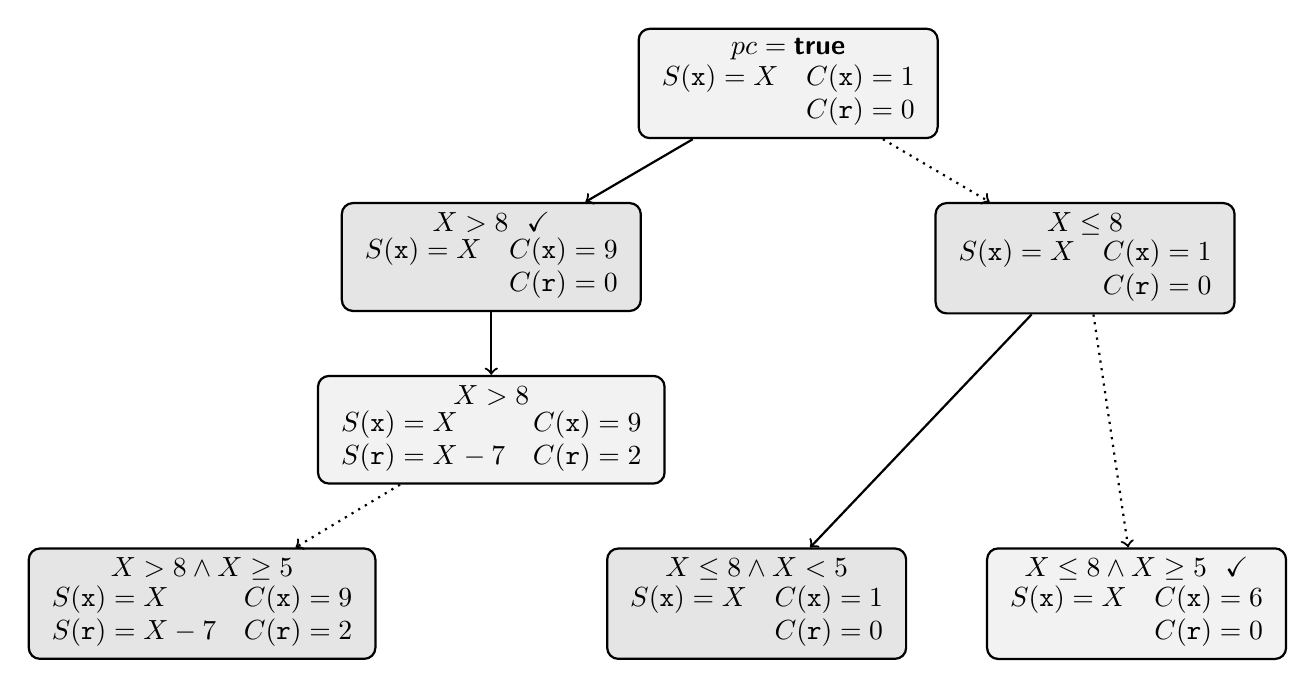
\begin{tikzpicture}[
        node distance=1.5cm and 1cm,
        every node/.style={draw, rounded corners, fill=gray!10, align=center},
        every path/.style={thick},
        decision/.style={draw, rounded corners, fill=gray!20, align=center, minimum width=3.5cm, yshift=2em}
    ]


    % Nodes
      \node (start) {\textbf{$pc = \textsf{true}$} \\
        $\begin{array}{ll}
        S(\mathtt{x}) = X & C(\mathtt{x}) = 1 \\
                          & C(\mathtt{r}) = 0
      \end{array}$ };
    
    \node (left)[below left=of start, decision,xshift=3em] {$X > 8 ~~ \checkmark$ \\ 
        $\begin{array}{ll}
        S(\mathtt{x}) = X & C(\mathtt{x}) = 9 \\
                          & C(\mathtt{r}) = 0
      \end{array}$ };
    \node (left2)[below=of left,yshift=2em] {$X > 8$ \\ 
        $\begin{array}{ll}
        S(\mathtt{x}) = X & C(\mathtt{x}) = 9 \\
        S(\mathtt{r}) = X - 7 & C(\mathtt{r}) = 2
      \end{array}$ };
    \node (left3)[below left=of left2,decision,xshift=5em] {$X > 8 \wedge X \ge 5$ \\ 
        $\begin{array}{ll}
        S(\mathtt{x}) = X & C(\mathtt{x}) = 9 \\
        S(\mathtt{r}) = X - 7 & C(\mathtt{r}) = 2
      \end{array}$ };
    
    \node (right)[below right=of start, decision,xshift=-3em] {$X \leq 8$ \\ 
        $\begin{array}{ll}
        S(\mathtt{x}) = X & C(\mathtt{x}) = 1 \\
                          & C(\mathtt{r}) = 0
      \end{array}$ };
    \node (right2)[below right=of left2,decision,xshift=-5em] {$X \le 8 \wedge X < 5$ \\ 
        $\begin{array}{ll}
        S(\mathtt{x}) = X & C(\mathtt{x}) = 1 \\
                          & C(\mathtt{r}) = 0
      \end{array}$ };
    \node (right2b)[right=of right2] {$X \le 8 \wedge X \ge 5 ~~ \checkmark$ \\ 
        $\begin{array}{ll}
        S(\mathtt{x}) = X & C(\mathtt{x}) = 6 \\
                          & C(\mathtt{r}) = 0
      \end{array}$ };
    
    % Edges
    \draw[->] (start) -- (left);
    \draw[->] (left) -- (left2);
    \draw[->,dotted] (left2) -- (left3);
    \draw[->] (right) -- (right2);
    \draw[->,dotted] (right) -- (right2b);
    \draw[->, dotted] (start) -- (right);
    
    \end{tikzpicture}
\end{center}
Finally, we finish unfinished business with the then-branch of (2) and run through the body of that conditional.
\begin{center}
    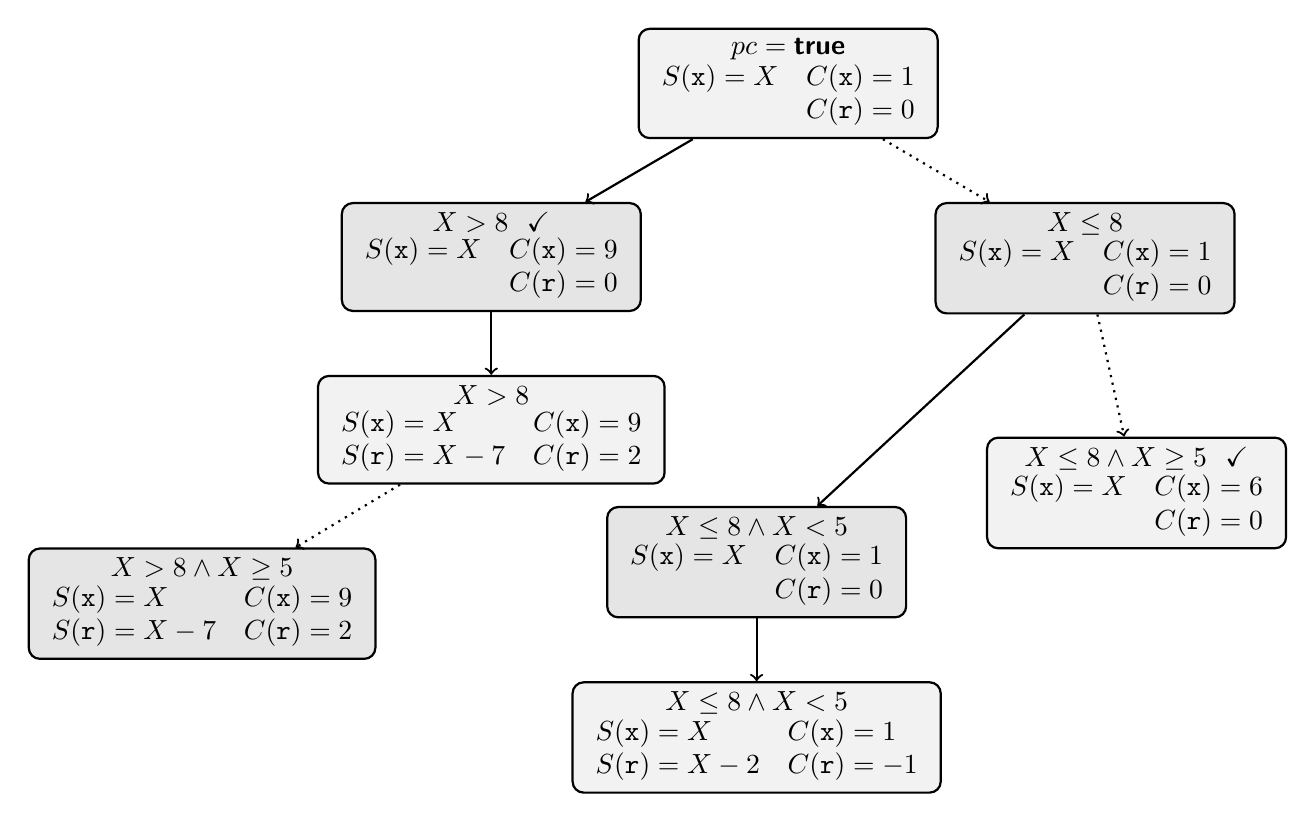
\begin{tikzpicture}[
        node distance=1.5cm and 1cm,
        every node/.style={draw, rounded corners, fill=gray!10, align=center},
        every path/.style={thick},
        decision/.style={draw, rounded corners, fill=gray!20, align=center, minimum width=3.5cm, yshift=2em}
    ]


    % Nodes
      \node (start) {\textbf{$pc = \textsf{true}$} \\
        $\begin{array}{ll}
        S(\mathtt{x}) = X & C(\mathtt{x}) = 1 \\
                          & C(\mathtt{r}) = 0
      \end{array}$ };
    
    \node (left)[below left=of start, decision,xshift=3em] {$X > 8 ~~ \checkmark$ \\ 
        $\begin{array}{ll}
        S(\mathtt{x}) = X & C(\mathtt{x}) = 9 \\
                          & C(\mathtt{r}) = 0
      \end{array}$ };
    \node (left2)[below=of left,yshift=2em] {$X > 8$ \\ 
        $\begin{array}{ll}
        S(\mathtt{x}) = X & C(\mathtt{x}) = 9 \\
        S(\mathtt{r}) = X - 7 & C(\mathtt{r}) = 2
      \end{array}$ };
    \node (left3)[below left=of left2,decision,xshift=5em] {$X > 8 \wedge X \ge 5$ \\ 
        $\begin{array}{ll}
        S(\mathtt{x}) = X & C(\mathtt{x}) = 9 \\
        S(\mathtt{r}) = X - 7 & C(\mathtt{r}) = 2
      \end{array}$ };
    
    \node (right)[below right=of start, decision,xshift=-3em] {$X \leq 8$ \\ 
        $\begin{array}{ll}
        S(\mathtt{x}) = X & C(\mathtt{x}) = 1 \\
                          & C(\mathtt{r}) = 0
      \end{array}$ };
    \node (right2)[below right=of left2,decision,xshift=-5em,yshift=1.5em] {$X \le 8 \wedge X < 5$ \\ 
        $\begin{array}{ll}
        S(\mathtt{x}) = X & C(\mathtt{x}) = 1 \\
                          & C(\mathtt{r}) = 0
      \end{array}$ };
    \node (right21)[below=of right2,yshift=2em] {$X \le 8 \wedge X < 5$ \\ 
        $\begin{array}{ll}
        S(\mathtt{x}) = X & C(\mathtt{x}) = 1 \\
        S(\mathtt{r}) = X-2 & C(\mathtt{r}) = -1
      \end{array}$ };
    \node (right2b)[right=of right2,yshift=2.5em] {$X \le 8 \wedge X \ge 5 ~~ \checkmark$ \\ 
        $\begin{array}{ll}
        S(\mathtt{x}) = X & C(\mathtt{x}) = 6 \\
                          & C(\mathtt{r}) = 0
      \end{array}$ };
    
    % Edges
    \draw[->] (start) -- (left);
    \draw[->] (left) -- (left2);
    \draw[->,dotted] (left2) -- (left3);
    \draw[->] (right) -- (right2);
    \draw[->] (right2) -- (right21);
    \draw[->,dotted] (right) -- (right2b);
    \draw[->, dotted] (start) -- (right);
    
    \end{tikzpicture}
\end{center}
We have satisfying assignments $X = 9$, $X = 1$, and $X = 6$, yielding test cases
\texttt{proc(9)}, \texttt{proc(1)}, \texttt{proc(6)}.

\paragraph{EXE: Implementation considerations.} An implementation of EXE needs to maintain multiple execution states while running the program, with both
symbolic and concrete components. As we saw, we need to switch back and forth between different program points and states. The answer is a special-purpose virtual machine.

KLEE (\url{klee.github.io}) uses the LLVM bitcode interpreter to maintain and update state. This means that programs to be run under KLEE need to be compiled into LLVM bitcode.
You can't compile everything into bitcode though, especially assembly, system calls, and some third-party libraries.

S$^2$E (\url{s2e.systems}) instead uses the QEMU virtual machine to fork and restore the entire machine state, including the operating system. It can therefore execute everything.
It executes any code from the executable of interest symbolically. There's still the problem with system code (the code that couldn't be compiled into bitcode), and it runs that
code concretely. Under-the-hood, it uses LLVM.

\section{DART: Directed Automated Random Testing}

\bibliographystyle{alpha}
\bibliography{L09}

\end{document}
